\begin{definition}{Vektor}
    Ein Vektor ist ein Objekt, das einen \textit{Betrag} (Länge) und eine \textit{Richtung} hat.
    Vektoren werden durch Kleinbuchstaben mit einem Pfeil darüber bezeichnet ($\vec{a}$).
    Der Vektor, der den Punkt $P$ in $Q$ verschiebt, wird als $\vec{PQ}$ bezeichnet.
    Beschreiben zwei Vektoren dieselbe Translation (selber Betrag und Richtung),
    werden sie als gleich betrachtet.
    Es wird zwischen \textit{Orts-} und \textit{Richtungsvektoren} unterschieden.
\end{definition}

\begin{definition}{Nullvektor}\\
    Der Vektor mit dem Betrag $0$ (es gibt nur einen) heisst \textit{Nullvektor} und wird mit $\vec{0}$ bezeichnet.
    Der Nullvektor ist der \textbf{einzige Vektor ohne Richtung}.
\end{definition}

\begin{definition}{Einheitsvektor}\\
    Ein Vektor mit Betrag $1$ heisst \textit{Einheitsvektor} oder normiert und wird mit $\vec{e}$ bezeichnet 
    (evtl. mit einem Index zwecks Unterscheidung von anderen Einheitsvektoren: z. B. $\vec{e_a}$). 
\end{definition}

\begin{definition}{Länge/Betrag eines Vektors}\\
    Der Betrag eines Vektors ist gegeben durch:
    \begin{equation*}
        \abs{\vec{a}}=\sqrt{a_1^2+a_2^2+\cdots+a_n^2}
    \end{equation*}
\end{definition}

\begin{formula}{Berechnung Einheitsvektor/normieren}
    Gegeben ein Vektor $\vec{a}$ mit Betrag $a=\abs{\vec{a}}$. 
    So ist der Einheitsvektor ist gegeben durch:
    \begin{equation*}
        \vec{e_a}=\frac{1}{a}\cdot\vec{a}
    \end{equation*}
    Der Vektor $\vec{e_a}$ wird als \textbf{Einheitsvektor oder auch normiert} bezeichnet 
    und der Übergang von $\vec{a}$ nach $\vec{e_a}$ heisst \textbf{Normierung}.
\end{formula}

\begin{theorem}{Rechenregeln für Vektoren I}\\
    Für beliebige Vektoren $\vec{a}, \vec{b}$ und $\vec{c}$ gilt:
    \begin{center}
        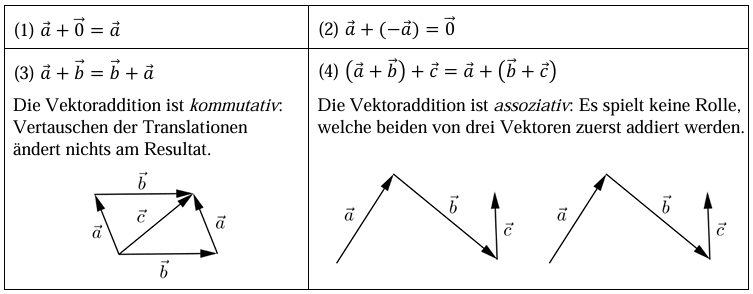
\includegraphics[width=0.8\linewidth]{images/vec-calc-regeln.png}
    \end{center}
\end{theorem}

\begin{theorem}{Rechenregeln für Vektoren II}
    \begin{itemize}
        \item $(-\lambda)\cdot\vec{a}=-(\lambda\cdot\vec{a})=\lambda\cdot(-\vec{a})$
        \item Assoziativ-Gesetz $\lambda\cdot(\mu\cdot\vec{a})=(\lambda\cdot\mu)\cdot\vec{a}$ 
        \item Distributiv-Gesetz $(\lambda+\mu)\cdot\vec{a}=\lambda\vec{a}+\mu\vec{a}$
        \item Distributiv-Gesetz $\lambda\cdot(\vec{a}+\vec{b})=\lambda\cdot\vec{a}+\lambda\cdot\vec{b}$
    \end{itemize}
\end{theorem}

\begin{definition}{Normalenvektor}
    Ein Normalenvektor, der orthogonal zu einer Ebene $E$ ist, heisst \textit{Normalenvektor} von $E$.
    Eine Koordinatendarstellung einer Ebene $E$ heisst normiert, wenn gilt: $\vec{n}=1$.
\end{definition}

\begin{definition}{Gegenvektor}
    \begin{wrapfigure}{r}{0.2\linewidth}
        \vspace{-10pt}
        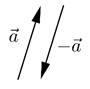
\includegraphics[width=0.6\linewidth]{images/vec-gegen.png}
    \end{wrapfigure}
    Der Vektor, der zu einem vorgegebenen Vektor $\vec{a}$ parallel ist und denselben Betrag,
    aber entgegengesetzte Richtung hat, heisst \textit{Gegenvektor} zu $\vec{a}$ und wird mit $-\vec{a}$ bezeichnet.
\end{definition}

\begin{definition}{Linearkombination}
    Gegeben sind $n$-Vektoren $\vec{a_1},\vec{a_2},\ldots,\vec{a_n}$.
    Der Ausdruck
    \begin{equation*}
        \lambda_1\cdot\vec{a_1}+\lambda_2\cdot\vec{a_2}+\ldots+\lambda_n\cdot\vec{a_n}
    \end{equation*}
    mit $\lambda_n\in R$ heisst \textit{Linearkombination} der Vektoren $\vec{a_1},\ldots,\vec{a_n}$.
\end{definition}

\begin{definition}{Kollinear}
    \begin{wrapfigure}{r}{0.2\linewidth}
        \vspace{-10pt}
        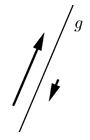
\includegraphics[width=0.6\linewidth]{images/vec-kollinear.png}
    \end{wrapfigure}
    Zwei Vektoren $\vec{a}$ und $\vec{b}$ heissen \textbf{kollinear}, 
    wenn es eine Gerade $g$ gibt, zu denen beide parallel sind. 
    Ein \textbf{Spezialfall} bildet dabei der Nullvektor, welcher zu jedem Vektor kollinear ist.
\end{definition}

\begin{theorem}{Eigenschaften kollinear Vektoren}\\
    Sind zwei Vektoren $\vec{a}$ und $\vec{b}$ kollinear, so ist einer ein Vielfaches des anderen; 
    es gibt also eine reelle Zahl $\lambda$, sodass gilt: 
    \begin{equation*}
        \vec{a}=\lambda\cdot\vec{b}
    \end{equation*}
\end{theorem}

\begin{definition}{Komplanar}
    \begin{wrapfigure}{r}{0.2\linewidth}
        \vspace{-10pt}
        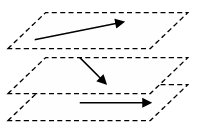
\includegraphics[width=\linewidth]{images/vec-komplanar.png}
    \end{wrapfigure}
    Drei Vektoren $\vec{a}$, $\vec{b}$ und $\vec{c}$ heissen \textbf{komplanar}, 
    wenn es eine Ebene $E$ gibt, zu denen alle drei parallel sind.
    \vspace{5pt}
\end{definition}

\begin{theorem}{Eigenschaften komplanarer Vektoren}\\
    \begin{wrapfigure}{r}{0.2\linewidth}
        \vspace{-10pt}
        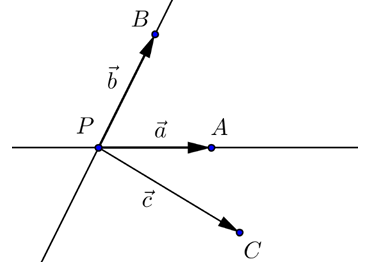
\includegraphics[width=\linewidth]{images/vec-kompl.png}
    \end{wrapfigure}
    Gegeben sind drei Vektoren $\vec{a}$, $\vec{b}$ und $\vec{c}$, für die gilt:
    \begin{itemize}
        \item $\vec{a}$, $\vec{b}$ und $\vec{c}$ sind komplanar.
        \item $\vec{a}$ und $\vec{b}$ sind nicht kollinear.
    \end{itemize} 
    Dann lässt sich $\vec{c}$ als Linearkombination von $\vec{a}$ und $\vec{b}$ darstellen; 
    es gibt also reelle Zahlen $\lambda$ und $\mu$, sodass gilt:
    \begin{equation*}
        \vec{c}=\lambda\cdot\vec{a}+\mu\cdot\vec{b}
    \end{equation*}
\end{theorem}

\begin{theorem}{Eigenschaften nicht komplanarer Vektoren}\\
    \begin{wrapfigure}{r}{0.2\linewidth}
        \vspace{-10pt}
        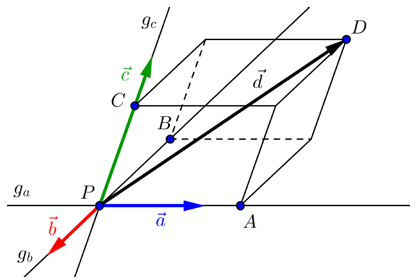
\includegraphics[width=\linewidth]{images/vec-nicht-kompl.png}
    \end{wrapfigure}
    Sind drei \textit{nicht komplanare} Vektoren $\vec{a}, \vec{b}$ und $\vec{c}$,
    dann lässt sich jeder Vektor $\vec{d}$ im $\R^3$ als Linearkombination von $\vec{a},\vec{b}$ und $\vec{c}$
    eindeutig darstellen;
    es gibt also reelle Zahlen $\lambda, \mu$ und $\nu$, so dass gilt:
    \begin{equation*}
        \vec{d}=\lambda\cdot\vec{a}+\mu\cdot\vec{b}+\nu\cdot\vec{c}
    \end{equation*}
\end{theorem}

\begin{definition}{Komponentendarstellung}\\
    Jeder Vektor $\vec{a}$ kann als Linearkombination von $\vec{e}_1, \vec{e}_2,\ldots\vec{e}_n$
    eindeutig dargestellt werden. 
    Es gibt reelle Zahlen $a_1, a_2, \ldots a_n$ genannt (Komponente), so dass gilt:
    \begin{equation*}
        \vec{a}=a_1\cdot\vec{e}_1+a_2\cdot\vec{e}_2+\cdots+a_n\cdot\vec{e}_n=
        \begin{psmallmatrix}
            a_1\\a_2\\\vdots\\a_n
        \end{psmallmatrix}
    \end{equation*}
\end{definition}

\begin{definition}{Ortsvektor}\\
    Zu jedem Punkt $P$ des Vektorraums ist ein \textit{Ortsvektor} definiert
    \begin{equation*}
        \vec{r}(P)=\overrightarrow{OP}
    \end{equation*}.
    Ortsvektoren sind im Ursprung $O$ angeheftet und sind wie jeder Vektor Linearkombination 
    von $\vec{e_1}, \vec{e_2},\ldots, \vec{e_n}$ und lassen sich in Komponentenschreibweise darstellen:
    \begin{equation*}
        \vec{r}(P)=x_1\cdot\vec{e}_1+x_2\cdot\vec{e}_2,\ldots,x_n\cdot\vec{e}_n,\, \text{ also }
        \begin{psmallmatrix}
            x_1\\x_2\\\vdots\\x_n
        \end{psmallmatrix}
    \end{equation*}
\end{definition}

\begin{formula}{Komponentendarstellung von $\overrightarrow{OP}$}\\
    \vspace{-20pt}
    \begin{wrapfigure}{r}{0.3\linewidth}
        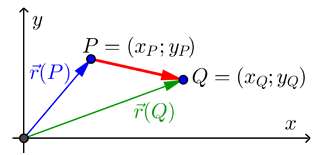
\includegraphics[width=\linewidth]{images/vec-komp-calc.png}
    \end{wrapfigure}
    \begin{align*}
        \vec{r}(Q)                      &=\vec{r}(P)+\overrightarrow{PQ}\\
        \Rightarrow \overrightarrow{PQ} &=\vec{r}(Q)-\vec{r}(P)=\begin{psmallmatrix}
            x_Q-x_P\\
            y_Q-y_P\\
            \cdots-\cdots
        \end{psmallmatrix}
    \end{align*}
\end{formula}

\begin{formula}{Rechnen mit Vektoren in Komponentendarstellung}\\
    Gegeben sind zwei Vektoren $\vec{a}=\begin{psmallmatrix}a_1\\a_2\\a_3\end{psmallmatrix}$
    und $\vec{b}=\begin{psmallmatrix}a_1\\a_2\\a_3\end{psmallmatrix}$ sowie ein $\lambda \in\R$.
    \begin{center}
        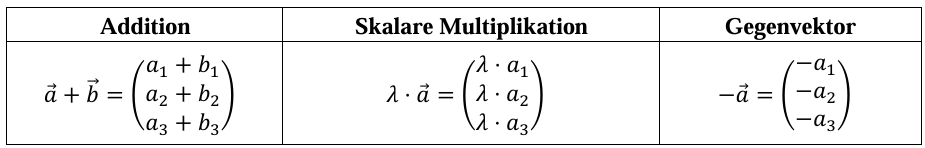
\includegraphics[width=\linewidth]{images/vec-komp-calc-regeln.png}
    \end{center}
\end{formula}